%----------------------------------------------------------------------------------------------------------------------------------------------------------%
\chapter{Physical experimentation}
\epigraph{A scientist in his laboratory is not a mere technician: he is also a child confronting natural phenomena that impress him as though they were fairy tales.}{\textit{Marie Curie}}
%----------------------------------------------------------------------------------------------------------------------------------------------------------%
\section{Description}
\paragraph{}This experiment is designed to detect and evaluate the prevalence of \emph{Staphylococcus aureus} in a sample of students from our school. The process used involves extracting a sample from underneath a subject's nails by swabbing, cultivating that sample, and then observing the results of said culture to determine the presence or not of \emph{Staphylococcus aureus} as part of the subject's resident bacterial flora. Each sampling iteration of the process took less than two minutes to complete. However, all the safety measures and actions taken need more time to be taken care of properly; as well as taking into account the fact that cultivating is not a task that can be done in just a day, often needing two to three to fully grow.
\begin{figure}[h!] \centering \begin{subfigure}[b]{0.4\linewidth} 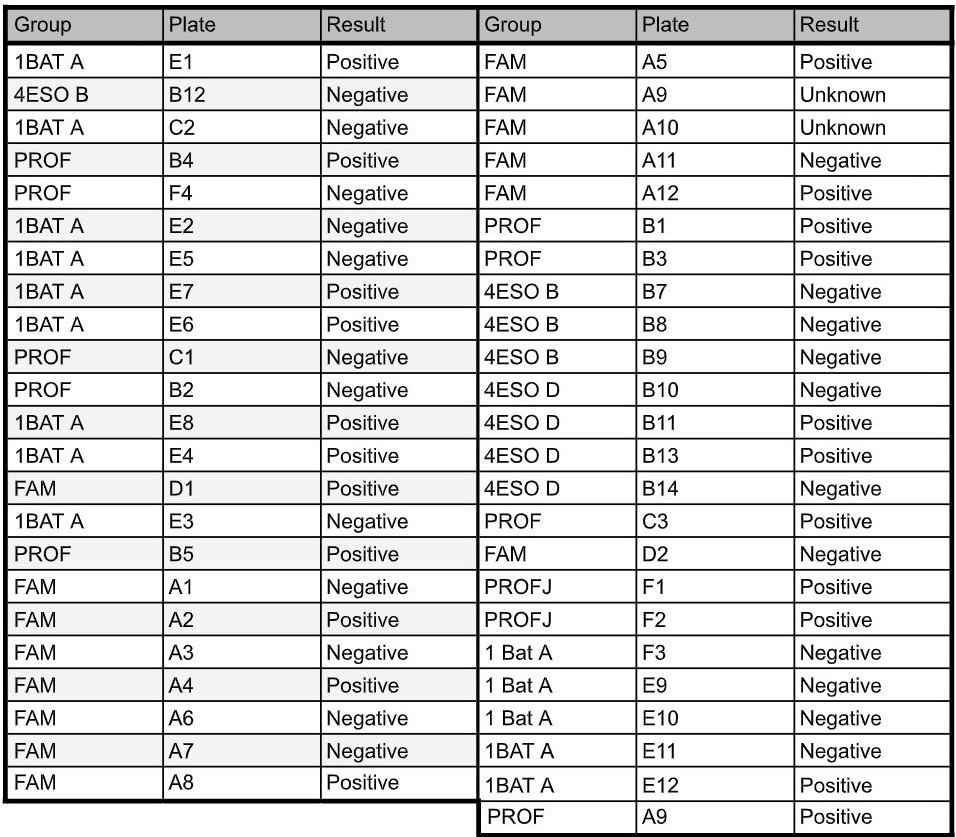
\includegraphics[width=\linewidth]{coffee.jpg} \caption{Coffee.} \end{subfigure} \begin{subfigure}[b]{0.4\linewidth} 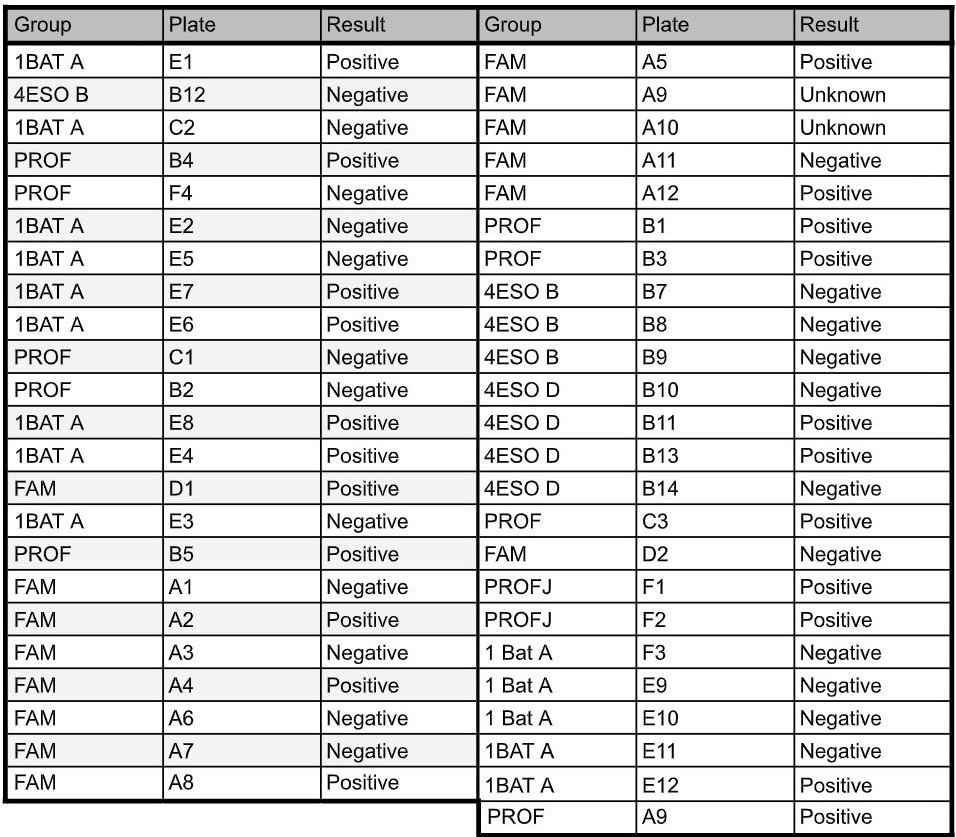
\includegraphics[width=\linewidth]{coffee.jpg} \caption{More coffee.} \end{subfigure} \caption{The same cup of coffee. Two times.} \label{fig:coffee}\end{figure}

%----------------------------------------------------------------------------------------------------------------------------------------------------------%
\section{Results and analysis}
The results obtained can be found in the following raw data table:
\begin{center}\begin{figure}[H]\centering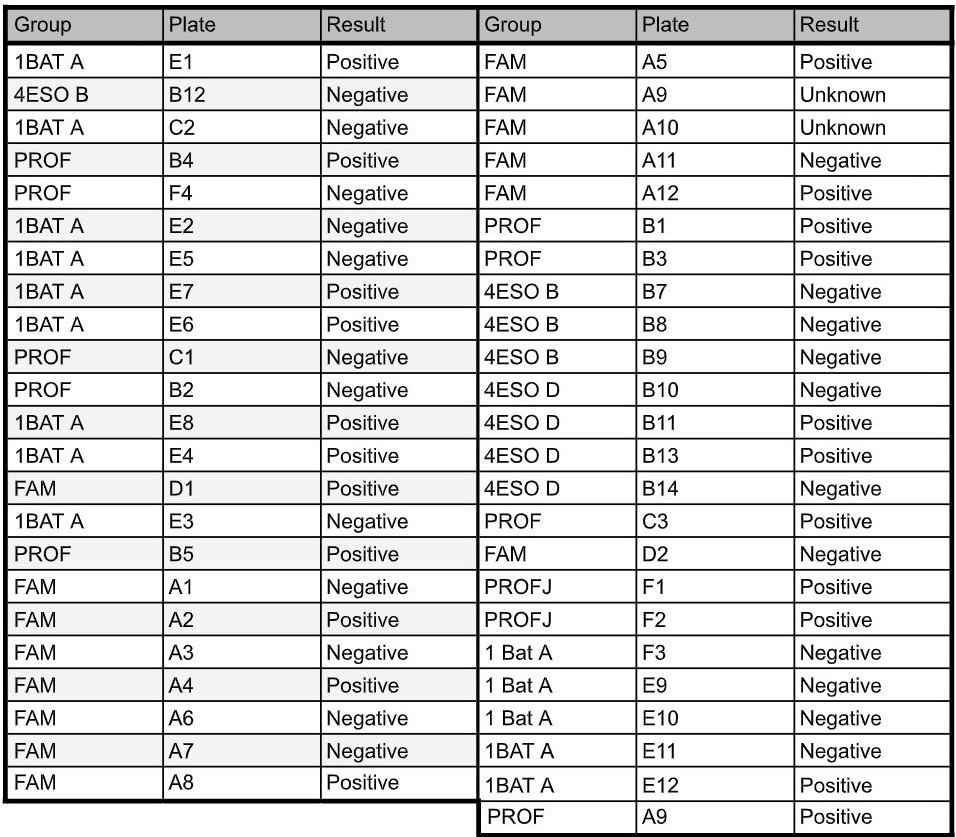
\includegraphics[width=0.80\textwidth]{RES-1.jpg}\end{figure}\end{center}
The data was then recounted and graphed into the following pie chart:
\begin{center}\begin{figure}[H]\centering\begin{subfigure}[b]{0.4\linewidth}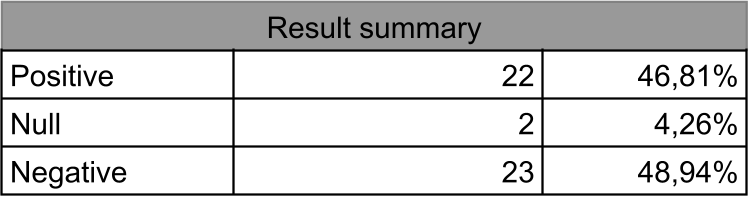
\includegraphics[width=0.95\linewidth]{Data.png}\caption{Counts of the result cases.}\end{subfigure}\begin{subfigure}[b]{0.38\linewidth}\includegraphics[width=0.95\linewidth]{Pie.png}\caption{Pie graph of the result cases.}\end{subfigure}\caption{Data processed from results}\end{figure}\end{center}\vspace{-1.5em}
As we can see, almost 50\% of the samples taken tested positive for \emph{Staphylococcus aureus}, compared to the expected 30\%\cite{StaphylococcusAureusHealthcare2020}. To confirm my results, I emailed two microbiology professors asking for their recent results on this kind of test, who had also found their experiments resulting in a higher prevalence than usual of this bacterium, as well as discovering cases that were previously negative but recently tested positive positive. Their results were not only confirmed by the detection of it by an MSA plate, but also by taking the morphological observation into account, both macroscopically and microscopically.
\begin{figure}[H]\centering\begin{subfigure}[b]{0.4\linewidth}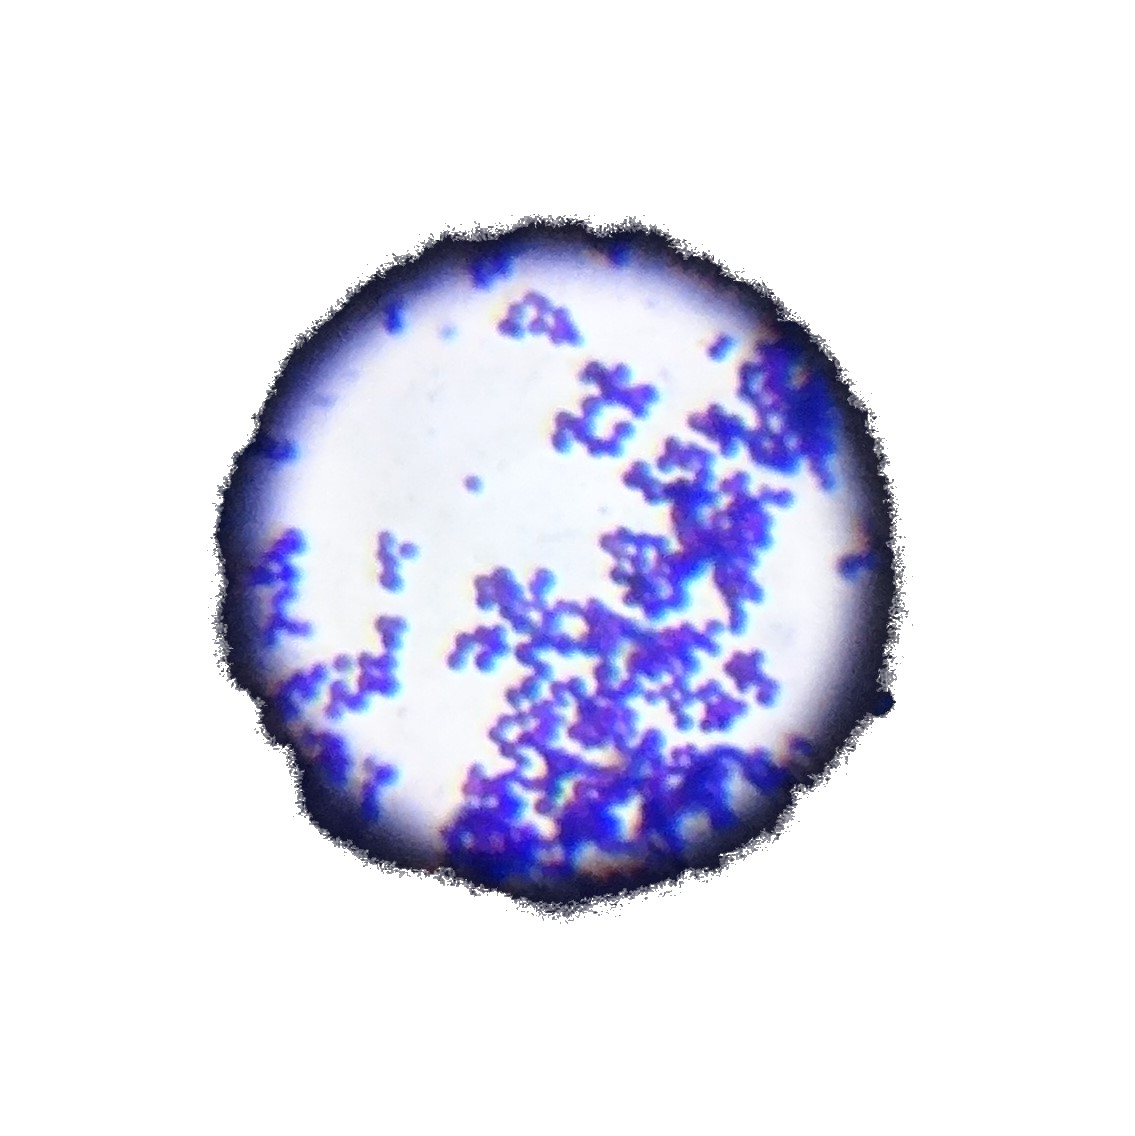
\includegraphics[width=\linewidth]{microscope.JPG}\caption{\emph{Staphylococcus aureus} as seen below the microscope. x4000, GRAM staining}\end{subfigure}\begin{subfigure}[b]{0.4\linewidth}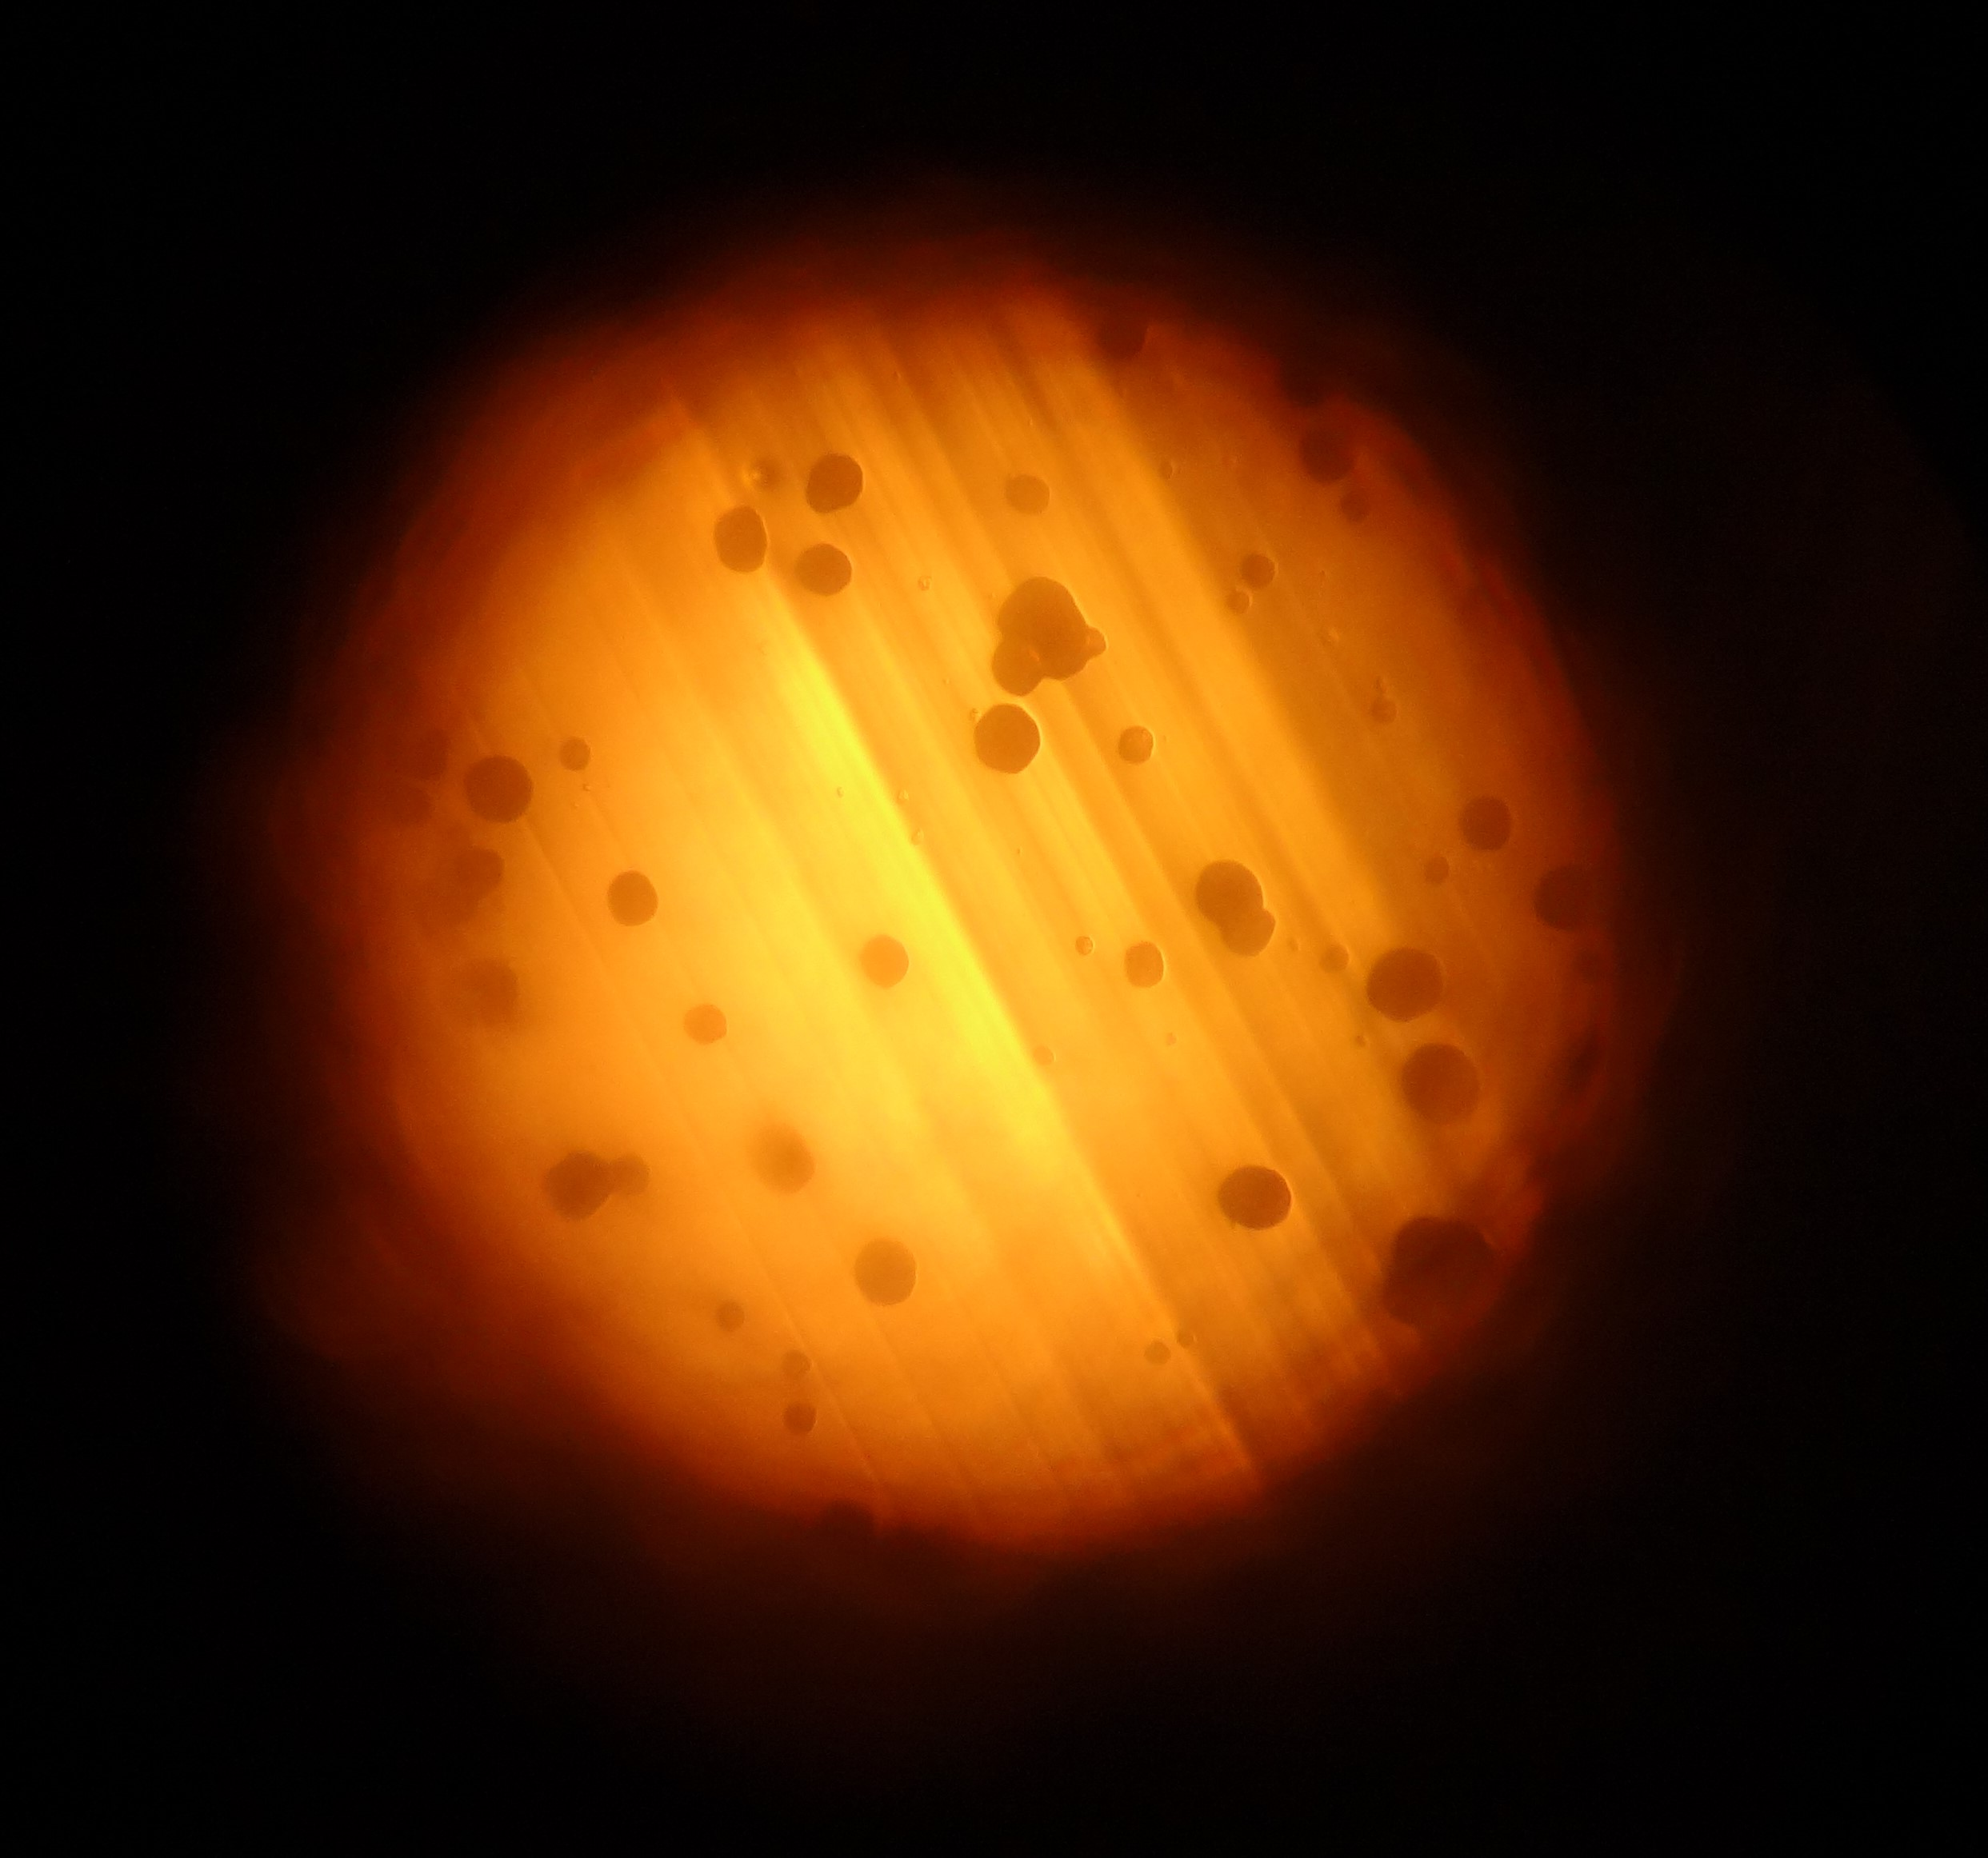
\includegraphics[width=\linewidth]{colonies.JPG}\caption{Colonies of \emph{Staphylococcus aureus} seen under a magnifying glass, x50, no staining}\end{subfigure}\caption{Photographies of the results, as collected from my own experimentation (own data).}\end{figure}
\paragraph{}There may be several reasons for the infection rate and thus natural prevalence to be increasing. One of them could be that since antibiotic abuse is growing with each passing year, the usual resident microbiota is getting killed, leaving more resources for Staph to thrive in that environment. To confirm this theory, we will look at the infection rates of a country that is facing extreme antibiotic abuse (the United States of America) and compare it to another that is controlling their antibiotics a bit better (the United Kingdom). The former have seen a 210\% increase in \emph{Staphylococcus aureus} cases since 2006. However, superfluous antibiotic prescriptions have increased by barely 1\%\cite{baggsEstimatingNationalTrends2016}. In the United Kingdom, they have seen a 160\% increase in \emph{Staphylococcus aureus} infections\cite{englandMSSABacteraemiaAnnual2021}, and their superfluous antibiotic prescriptions have gone down by 20\%. Even though this is very little data to extract conclusions from, there may be a correlation between these two factors.
\paragraph{}Let's compare the prevalence among different groups of subjects, starting with their gender.
\begin{center}\begin{figure}[H]\centering\begin{subfigure}[b]{0.4\linewidth}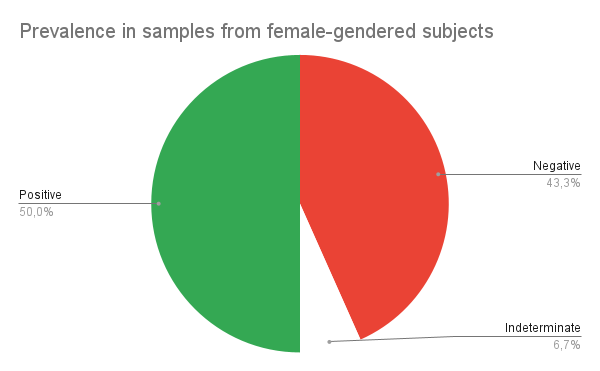
\includegraphics[width=0.95\linewidth]{gend_fem.png}\caption{Counts of the result cases in female-gendered individuals}\end{subfigure}\begin{subfigure}[b]{0.38\linewidth}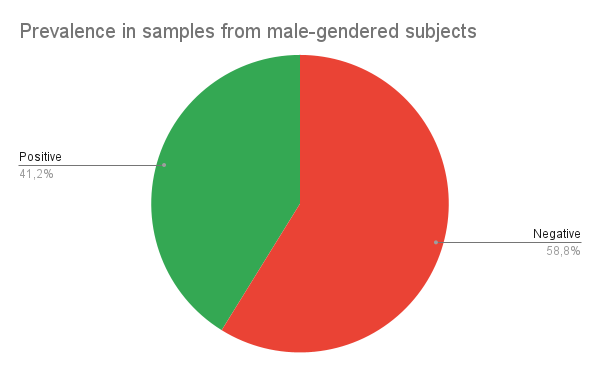
\includegraphics[width=0.95\linewidth]{gend_male.png}\caption{Counts of the result cases in male-gendered individuals}\end{subfigure}\caption{Data processed from results}\end{figure}\end{center}\vspace{-1.5em}
As we can observe, there is a 10\% difference in prevalence between these two genders. In my opinion, this is due to a small sample size. As we can see, the first graph, which houses the samples from subjects who identify themselves as female, has a third type of result, which the other graph, which houses the samples from subjects who self-identify as male, does not. This is simply due to a problem with the plates, however, it may affect the final result. I believe there to not be any significant difference between the two analyzed genders.
\begin{center}\begin{figure}[H]\centering\begin{subfigure}[b]{0.4\linewidth}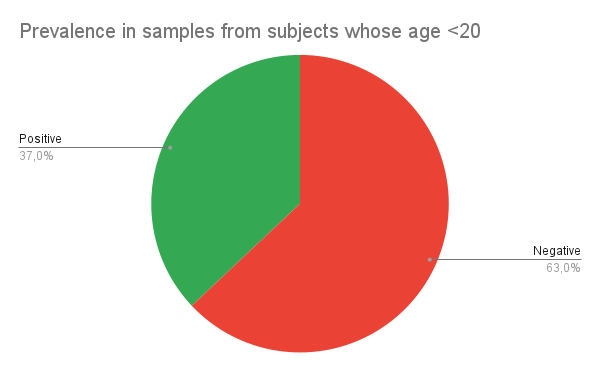
\includegraphics[width=0.95\linewidth]{age_young.png}\caption{Counts of the result cases in subjects younger than 20}\end{subfigure}\begin{subfigure}[b]{0.38\linewidth}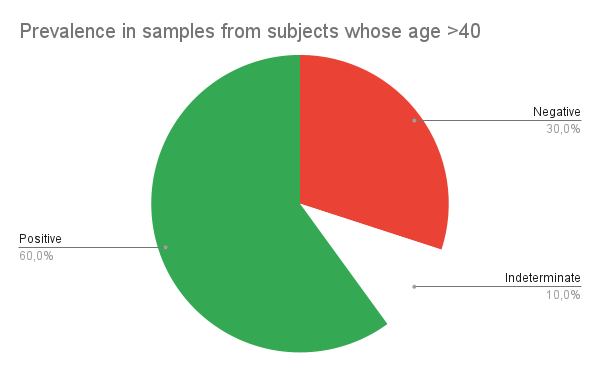
\includegraphics[width=0.95\linewidth]{age_old.png}\caption{Counts of the result cases in subjects older than 40}\end{subfigure}\caption{Data processed from results}\end{figure}\end{center}\vspace{-1.5em}
Only two age groups were studied, due to the fact that the samples fell mostly into one of these two categories. We can see that the samples from a subject older than 40 were twice as likely to test positive for \emph{Staphylococcus aureus} than those from subjects younger than 20. This may be due to a small sample size. However, it may also be possible that the possibility of hosting this bacterium increases with age. In order to confirm this theory, more studies should be done, with a greater age gradient, as well as many more samples. It may also be the case that this change in prevalence is not caused by one single variable, but due to multiple at the same time.
